         \chapter{Fases van materie en die kinetiese molekul\^{e}re teorie}\fancyfoot[LO,RE]{Chemistry: Matter and Materials}
    \setcounter{figure}{1}
    \setcounter{subfigure}{1}
% \label{m38736*cid1}
%             \section{ Introduction}
%             \nopagebreak
\label{m38736*cid2}
            \section{Fases van materie}
            \nopagebreak

\label{m38736*id802341}In hierdie hoofstuk verken ons die fases van materie en kyk dan na die kinetiese molekul\^{e}re teorie. Materie kom in drie toestande voor: vaste stof, vloeistof en gas. Ons ondersoek ook hoe die kinetiese teorie van die materie help om kook-en smeltpunte, asook ander eienskappe van materie, te verduidelik.\par 

\label{m38736*id324876121}Alle materie bestaan uit deeltjies. Ons kan dit sien as ons na diffusie kyk. \par
\Definition{Diffusie}{Diffusie is die beweging van deeltjies van 'n ho\"{e} konsentrasie na' n lae konsentrasie} 
\begin{minipage}{.5\textwidth}
Diffusie kan gesien word as 'n eweredige verspreiding van deeltjies. Jy kan diffusie sien wanneer jy 'n druppel voedselkleursel in die water sit. Die kleur versprei stadig deur die water. As materie nie uit deeltjies bestaan het nie sou ons net 'n kleurklont (opeenhoping van kleur) gesien het wanneer ons die voedselkleursel in die water sit, want daar sou niks gewees wat in die water rond kon beweeg en met die water meng nie.
\end{minipage}
\begin{minipage}{.5\textwidth}
\begin{center}
 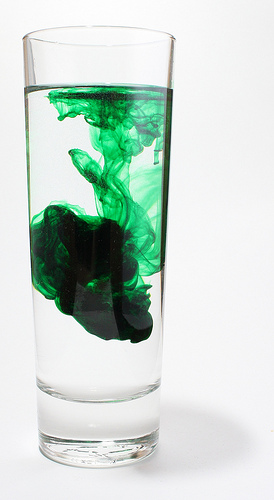
\includegraphics[height=.5\textwidth]{photos/diffusionby-LadyDayDream-flickr.jpg}\par
\textit{Picture by LadyDayDream on Flickr.com}
\end{center}
\end{minipage}

\par 
\label{m38736*id10987324}\textbf{Diffusie} is 'n gevolg van die konstante termiese beweging van deeltjies. In 1828 het Robert Brown waargeneem dat stuifmeelkorrels wat in water geplaas is, vinnige onreëlmatige bewegings uitvoer. Hierdie beweging het sedertdien bekend geword as \textbf{Brownbewegin}. . Brownbeweging is in wese die diffusie van baie deeltjies.
\par 
\label{m38736*id48327}Materie kom voor in een van drie toestande, naamlik vaste stof, vloeistof en gas. 'n Vaste stof het 'n vaste vorm en volume. 'n Vloeistof neem die vorm van die houer aan waarin dit is. 'n Gas vul heeltemal die houer waarin dit is. Materie kan tussen hierdie toestande verander deur óf byvoeging van hitte of die verwydering van hitte. Dit is bekend as 'n faseverandering. Soos ons 'n voorwerp (bv. water) verhit, verander dit van 'n vaste stof na 'n vloeistof na 'n gas. As ons 'n voorwerp afkoel, gaan dit van 'n gas na 'n vloeistof na 'n vaste stof. Die faseveranderings wat jy moet ken is:
\label{m38736*id02341}\begin{itemize}[noitemsep]
\item \textbf{Smelt} \\ 
\Definition{\label{id2412224} Smelt punt } { \label{m38734*meaningfhsst!!!underscore!!!id276}
Die temperatuur waarby 'n \textsl{vaste stof} sy fase of toestand verander om 'n \textsl{vloeistof} te word. Die proses staan bekend as smelt. } 
\item \textbf{Vries} \\
\Definition{Vries punt}{Die temperatuur waarby 'n \textsl{vloeistof} sy fase of toestand verander om 'n \textsl{vaste stof} te word. Die proses staan bekend as vries.}
\item \textbf{Verdamping} \\
Verdamping is die proses waar tydens 'n vloeistof oorgaan na 'n gas. Verdamping kan van die vloeistof \textbf{oppervlak} af plaasvind oor 'n wye reeks temperatuur. As meer energie toegevang word verskyn borreltjies gas \textbf{binne} die vloeistof - die proses staan bekend as kook.
\Definition{   \label{id2412302} Kook punt } { \label{m38734*meaningfhsst!!!underscore!!!id282}
Die spesifieke temperatuur waarby 'n \textsl{vloeistof} van fase verander om 'n \textsl{gas} te word.} 
\item \textbf{Kondensasie} is die teenoorgestelde van verdamping. Tydens hierdie oorgaansproses verander 'n gas na vloeistof.
\item \textbf{Sublimasie} is die proses waar tydens 'n vaste stof direk oorgaan na 'n gas. Die omgekeerde proses staan bekend as deposisie (neerslagvorming)\end{itemize}
\par \label{m38736*eip-957}As ons weet wat die smelt- en kookpunt van 'n stof is, dan kan ons s\^{e} in watter toestand (vaste, vloeibare of gas) dit sal wees by enige temperatuur. \par 
Die volgende diagram gee 'n opsomming van hierdie prosesse: \\
    \setcounter{subfigure}{0}
\begin{figure}[H]
\begin{center}
\scalebox{0.8}{
\begin{pspicture}(-2,-2)(15,15)
\SpecialCoor
%\psgrid[gridcolor=lightgray]
\uput[r](-1,1.6){\large{Gas}}
\psline[linewidth=1.5pt]{->}(0.5,2)(4,2)
\uput[r](0.8,2.4){\large{Kondensasie}}
\uput[r](4.2,1.6){\large{Vloeistof}}
\psline[linewidth=1.5pt]{->}(6,2)(9.5,2)
\uput[r](6.8,2.4){\large{Vries}}
\uput[r](9.8,1.6){\large{Vaste stof}}
\psline[linewidth=1.5pt]{<-}(0.5,1)(4,1)
\uput[r](0,0.4){\large{Kook (of verdamping)}}
\psline[linewidth=1.5pt]{<-}(6,1)(9.5,1)
\uput[r](6.8,0.4){\large{Smelt}}
\psline[linewidth=1.5pt]{<-}(0.5,-0.5)(9.5,-0.5)
\uput[r](4,-1){\large{Sublimasie}}
\end{pspicture}
}
\caption{Fase veranderinge}
\label{fig:PhaseChanges}
\end{center}
\end{figure} 

\nopagebreak
\label{m38736*eip-232}
            \begin{f_experiment}{Verhitting- en afkoelingskurwe van water}{           
            \label{m38736*eip-860}\noindent{}\textbf{Doel}
Om die verhitting- en afkoelingskurwe van water te ondersoek. \\
\par 
\label{m38736*eip-861}\noindent{}\textbf{Apparaat} \\
\begin{minipage}{0.25\textwidth}
\begin{itemize}[noitemsep]
 \item bekers
 \item ys
 \item Bunsenbrander
 \item termometer
 \item water
\end{itemize}
\end{minipage}
\begin{minipage}{0.75\textwidth}
\begin{figure}[H]
 \begin{center}
\scalebox{0.5}
{
  \begin{pspicture}(-5,-5)(5,5)
\psset{unit=1cm}
%\psgrid(0,0)(-5,-5)(5,5)
\newpsstyle{cyan} {linestyle=none,fillstyle=solid,fillcolor=cyan}
\newpsstyle{clear} {linestyle=none,fillstyle=solid,fillcolor=white}
%\uput[r](3.5,1){\large{boiling water}}
%\psline[linewidth=0.04]{->}(3.55,1)(2.6,1)
%\uput[r](3.5,3){\large{metal spoon}}
%\psline[linewidth=0.04]{->}(3.55,3)(3,3)
\rput(-4,0){\pstTubeEssais[glassType=becher,niveauLiquide1=20,solide={\pstGrenailleZinc[200]},aspectLiquide1=clear]}
\psline[linewidth=0.1](-4.7,-2)(-2,2)
\psline[linewidth=0.04]{<-}(-2.34,1.5)(-1.5,1.5)
\uput[r](-1.5,1.5){\large{Termometer}}
\psline[linewidth=0.04]{<-}(-3,-1)(-1.5,-1)
\uput[r](-1.5,-1){\large{Beker}}
\psline[linewidth=0.04]{<-}(-3.5,-1.5)(-1.5,-1.5)
\uput[r](-1.5,-1.5){\large{Ys}}
\rput(2,0){\pstTubeEssais[glassType=becher,niveauLiquide1=30,aspectLiquide1=cyan]}
\psline[linewidth=0.1](1.4,-2)(4,2)
\psline[linewidth=0.04]{<-}(3.7,1.5)(4.5,1.5)
\uput[r](4.5,1.5){\large{Termometer}}
\psline[linewidth=0.04]{<-}(3,-1)(4.5,-1)
\uput[r](4.5,-1){\large{Beaker}}
\psline[linewidth=0.04]{<-}(2.5,-1.5)(4.5,-1.5)
\uput[r](4.5,-1.5){\large{Water}}
\end{pspicture}
}
 \end{center}
\end{figure}
\end{minipage} \\
\label{m38736*eip-862}\noindent{}\textbf{Metode:}
\label{m38736*id9872}\begin{itemize}[noitemsep]
            \item Plaas 'n paar stukkies ys in 'n beker.
\item Meet die temperatuur van die ys en teken dit aan.
\item Meet die temperatuur weer na 1 minuut, en teken dit aan. Herhaal die proses vir ten minste tot 3 minute nadat die ys gesmelt het.
\item Trek 'n grafiek van die tyd teen die temperatuur vir die verhitting van ys. 
\item Verhit 'n bietjie water in 'n beker totdat dit kook. Meet en noteer die temperatuur van die water.
\item Verwyder die water van die hitte en meet die temperatuur elke 1 minuut, totdat die beker koel genoeg is om dit aan te raak.
\item Trek die grafiek van tyd teenoor temperatuur vir die afkoeling van kookwater. 
\end{itemize}
\label{m38736*eip-282}
      \Warning {Wees versigtig wanneer jy die beker met warm water hanteer. Moenie aan die beker met jou hande raak nie, jy mag brand.}
	\par 
      \label{m38736*eip-863}\noindent{}\textbf{Resultate} \\
\begin{enumerate}[noitemsep, label=\textbf{\arabic*}.]
\item Skryf jou resultate in die volgende tabel neer: \\
          \begin{table}[H]
        \begin{center}
      \label{m38736*uid434}
    \noindent
      \begin{tabular}{|l|l|l|l|}\hline
\multicolumn{2}{|c|}{Verhitting van ys} & \multicolumn{2}{|c|}{Afkoeling van kookwater}  \\ \hline
 \textbf{Tyd (min)} & \textbf{Temperatuur (in $^{\circ} C$)} &  \textbf{Tyd (min)} & \textbf{Temperatuur (in $^{\circ} C$)} \\ \hline
     0    & & 0    & \\ \hline 
     1    & & 1    & \\ \hline
     2    & & 2    & \\ \hline
     etc. & & etc. & \\ \hline
%           & &      & \\ \hline 
%           & &      & \\ \hline
    \end{tabular}
      \end{center}
\end{table}
\item Trek 'n grafiek van tyd (die onafhanklike veranderlike, x-as) teenoor temperatuur (afhanklike veranderlike, y-as) vir die smelt van ys en die afkoeling van kookwater.
\end{enumerate}
\par   
\label{m38736*eip-864}\noindent{}\textbf{Bespreking en gevolgtrekking}\\
Jy sal vind dat die temperatuur van die ys toeneem totdat die eerste druppels vloeistof
verskyn; dan bly die temperatuur dieselfde (konstant) totdat al die ys gesmelt het. Jy sal ook
vind dat wanneer jy kookwater afkoel, die temperatuur vir 'n rukkie konstant bly voordat dit
begin afneem.}
\end{f_experiment} 
\par \label{m38736*eip-25}In die bostaande eksperiment het jy die verhittings- en afkoelingskurwes van water ondersoek. Ons kan
verhittings- en afkoelingskurwes vir enige stof trek. 'n Verhittingskurwe van 'n stof gee die veranderinge
in temperatuur aan soos die stof van 'n vaste stof na 'n vloeistof na 'n gas oorgaan. 'n Afkoelingskurwe gee
die veranderinge in temperatuur soos die stof van ‘n gas na vloeistof na‘n vaste stof oorgaan. 'n Belangrike
waarneming is dat wanneer 'n stof smelt of kook, die temperatuur konstant bly totdat die stof van fase verander
het. Dit is omdat al die hitte-energie gebruik word vir die verbreking of vorming van die kragte tussen die molekules.  \par 
Die volgende diagram is 'n voorbeeld van hoe verhittings- en afkoelingskurwes lyk: \par
\begin{minipage}{0.5\textwidth}
\begin{figure}[H]
 \begin{center}
\scalebox{0.3}{
  \begin{pspicture}
\psset{unit=1cm}
\psaxes[linewidth=1.2pt,labels=none,ticks=none]{->}(13,10)
\psline[linewidth=0.1](0,0)(2,2)(4,2)(10,8)(12,8)
\psaxes[linewidth=1.2pt,labels=none,ticks=none]{->}(13,10)
\rput[l]{0}(3,-0.5){\Huge{Tyd (min)}}
\rput[b]{90}(-0.5,5){\Huge{Temperatuur ($^{\circ} C$)}}
   \end{pspicture}
}
\end{center}
\caption{Verhittingskurwe}
\end{figure}
\end{minipage}
\begin{minipage}{0.5\textwidth}
\begin{figure}[H]
\begin{center}
\scalebox{0.3}{
  \begin{pspicture}
\psset{unit=1cm}
\psaxes[linewidth=1.2pt,labels=none,ticks=none]{->}(13,10)
\psline[linewidth=0.1](0,8)(2,8)(8,2)(10,2)(12,0)
\psaxes[linewidth=1.2pt,labels=none,ticks=none]{->}(13,10)
\rput[l]{0}(3,-0.5){\Huge{Tyd (min)}}
\rput[b]{90}(-0.5,5){\Huge{Temperatuur ($^{\circ} C$)}}
   \end{pspicture}
}
 \end{center}
\caption{Afkoelingskurwe}
\end{figure}
\end{minipage}
\end{fexperiment}
\label{m38736**end}

% \label{m38734*eip-661}
%     \setcounter{subfigure}{0}
% 	\begin{figure}[H] % horizontal\label{m38734*slidesharefigure1}
%     \label{m38734*slidesharemedia1}\label{m38734*slideshareflash1}
%             \raisebox{-5 pt}{ 
\includegraphics[width=0.5cm]{col11305.imgs/summary_www.png}} { (Presentation:  P10016 )}
%       \vspace{2pt}
%     \vspace{.1in}
%  \end{figure}       \par 
% \label{m38734**end}
         \section{Die kinetiese molekul\^{e}re teorie}
    \nopagebreak

%     \label{m38730*cid5}
%             \subsection{ The Kinetic Theory of Matter}
%             \nopagebreak
      \label{m38730*id308618}Die \textbf{kinetiese teorie} van materie help ons om te verduidelik waarom materie in verskillende fases voorkom (vaste, vloeistof en gas), en hoe materie kan oorgaan van een fase na die volgende. Die kinetiese teorie van materie help ons ook om ander eienskappe van materie te verstaan. Dit is belangrik om te besef dat wat ons gaan beskryf, slegs 'n \textsl{teorie}. Dit kan nie bo alle twyfel bewys word nie, maar die feit dat dit ons help om waarnemings van fase-verandering en ander eienskappe van materie te verduidelik, dui daarop dat dit waarskynlik meer as net 'n teorie is.
\par 
      \label{m38730*id308641}In die algemeen word die kinetiese teorie van materie gestel as:
\par 
      \label{m38730*id308647}\begin{itemize}[noitemsep]
            \label{m38730*uid34}\item Materie bestaan uit \textbf{deeltjies} wat voortdurend in beweging is.
\label{m38730*uid35}\item Alle deeltjies het \textbf{energie}. Vaste stof-deeltjies het die minste hoeveelheid energie en gasdeeltjies
het die grootste hoeveelheid energie.
\label{m38730*uid36}\item Die \textbf{temperatuur} van 'n stof is 'n maatstaf  van die \textsl{gemiddelde kinetiese energie} van die deeltjies.
\label{m38730*uid37}\item 'n Verandering in \textbf{fase} kan voorkom wanneer die energie van die deeltjies verander.
\label{m38730*uid38}\item Daar is \textbf{ruimtes} (spasies) tussen die deeltjies van materie.
\label{m38730*uid39}\item Daar is \textbf{aantrekkingskragte} tussen die deeltjies en hierdie aantrekkingskragte word sterker as die deeltjies nader aan mekaar beweeg.
\end{itemize}
      \label{m38730*id308767}Tabel \ref{tab:microscopic:kinetic theory} gee 'n opsomming van die eienskappe van die deeltjies in elke fase van materie.\par 
    % \textbf{m38730*uid40}\par
\begin{table}[h]
\begin{center}
\caption{Tabel met opsomming van die algemene eienskappe van die vaste stowwe, vloeistowwe en gasse.}
\label{tab:microscopic:kinetic theory}
\begin{tabular}{|p{3cm}|p{3cm}|p{3cm}|p{3cm}|}\hline
\textbf{Eienskap van materie} & \textbf{Vaste stof} & \textbf{Vloeistof} & \textbf{Gas} \\\hline
Deeltjies & Atome of molekules & Atome of molekules & Atome of molekules \\\hline
Energie en beweging van deeltjies & Min energie - deeltjies vibreer om'n vaste punt & Deeltjies het meer energie as in die vaste stof & Deeltjies het baie energie en is voortdurend aan die beweeg.  \\\hline
Spasies tussen  deeltjies & Baie min ruimte tussen deeltjies. Deeltjies is styf teenmekaar gepak. & Groter spasies as in die vaste stof fase. & Groot spasies a.g.v. ho\"{e} energie.  \\\hline
Aantrekkingskragte tussen deeltjies & Baie sterk kragte. Vaste stowwe het ‘n vaste volume. & Swakker kragte as in vaste stowwe, maar sterker as in gasse. & Swak kragte a.g.v. groot afstande. \\\hline
Fase-verandering & Vaste stowwe gaan oor in vloeistowwe of gasse. & 'n Vloeistof gaan oor in 'n gas as die temperatuur toeneem. Dit word 'n vaste stof as die temperatuur afneem. & Oor die algemeen word 'n gas 'n vloeistof of 'n vaste stof as dit afkoel. Die temperatuur toeneem. Deeltjies het minder energie en beweeg nader aan mekaar, sodat die aantrekkingskragte sterkter word en die gas verander in ‘n vloeistof of vaste stof.  \\\hline
\end{tabular}
\end{center}
\end{table}
    \par
%       \label{m38730*eip-933}The following presentation is a brief summary of the above. Try to fill in the blank spaces before clicking onto the next slide.
%     \setcounter{subfigure}{0}
% 	\begin{figure}[H] % horizontal\label{m38730*slidesharefigure}
%     \label{m38730*slidesharemedia}\label{m38730*slideshareflash}\raisebox{-5 pt}{ 
\includegraphics[width=0.5cm]{col11305.imgs/summary_www.png}} { (Presentation:  P10018 )}
%       \vspace{2pt}
%     \vspace{.1in}
%  \end{figure}       \par 
\begin{figure}[H]
\begin{center}
\begin{pspicture}(0,0)(10,2.6)
\SpecialCoor
%\psgrid[gridcolor=lightgray]

\rput(0,0.5){\psframe(0,0)(3,2)
\rput(0.1,0){\multirput(0.2,0.2)(0.4,0){7}{\pscircle(0,0){0.2}}
\multirput(0.4,0.55)(0.4,0){6}{\pscircle(0,0){0.2}}
\multirput(0.2,0.9)(0.4,0){7}{\pscircle(0,0){0.2}}}}

\rput(3.5,0.5){\psframe(0,0)(3,2)
\rput(0.2,0.2){\pscircle(0,0){0.2}}
\rput(0.6,0.3){\pscircle(0,0){0.2}}
\rput(1.2,0.3){\pscircle(0,0){0.2}}
\rput(1.7,0.2){\pscircle(0,0){0.2}}
\rput(2.3,0.3){\pscircle(0,0){0.2}}
\rput(2.8,0.2){\pscircle(0,0){0.2}}
\rput(0.3,0.9){\pscircle(0,0){0.2}}
\rput(0.8,0.7){\pscircle(0,0){0.2}}
\rput(1.5,0.8){\pscircle(0,0){0.2}}
\rput(2.0,0.8){\pscircle(0,0){0.2}}
\rput(2.5,0.7){\pscircle(0,0){0.2}}}

\rput(7,0.5){\psframe(0,0)(3,2)
\rput(2.5,0.5){\pscircle(0,0){0.2}}
\rput(2.4,1.7){\pscircle(0,0){0.2}}
\rput(1.5,1){\pscircle(0,0){0.2}}
\rput(0.7,1.7){\pscircle(0,0){0.2}}
\rput(0.3,0.3){\pscircle(0,0){0.2}}}

\uput[d](1.5,0.5){Vaste stof}
\uput[d](5,0.5){Vloeistof}
\uput[d](8.5,0.5){Gas}

\end{pspicture}
\end{center}
\caption{Die drie fases van materie}
\label{fig:threephases}
\end{figure}
      \label{m38730*id309053}Neem koper as voorbeeld. Ons vind dat koperatome min energie het in die vaste stof fase. Hulle vibreer in vaste posisies. Die atome is dig (styf) teen mekaar gepak in 'n reëlmatige, ordelike patroon, bekend as 'n \textsl{kristallyne rooster}. As koper verhit word, neem die energie van die atome toe. Dit beteken dat sommige van die koperatome in staat is om die kragte wat hulle saam hou te oorkom en hulle beweeg weg van mekaar om \textsl{vloeibare koper} te vorm. Vloeibare koper kan vloei, want die atome beweeg meer vrylik as wanneer hulle in die vaste rooster is. As die vloeistof verder verhit word, sal dit 'n gas word. Gasdeeltjies het baie energie en is ver weg van mekaar. Dit is waarom dit moeilik is om 'n gas in 'n spesifieke plek te hou! Die aantrekkingskragte tussen die deeltjies is baie swak. Gas-atome vul die houer waarin hulle is. Figuur~\ref{fig:PhaseChanges} toon die fase-veranderinge van materie, en die terminologie (name) wat hierdie prosesse beskryf.\par 
    \setcounter{subfigure}{0}
    
\begin{activity}{Die drie fases van water}
\begin{minipage}{0.5\textwidth}
Water kom voor as stoom, water (vloeistof) of ys. Gebruik albasters (of rol speelklei in klein balletjies) om watermolekules voor te stel. Rangskik die albasters om die drie fases van water aan te toon. Bespreek die eienskappe van elk van die fases, die betrokke prosesse en die energie-aspekte wanneer daar van een fase na ‘n ander oorgegaan word.
\end{minipage}
\begin{minipage}{.5\textwidth}
\begin{center}
 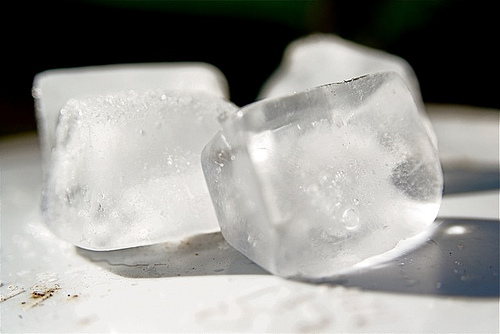
\includegraphics[width=.3\textwidth]{photos/iceby-stevendepolo-flickr.jpg}\par
\textit{Picture by stevendepolo on Flickr.com}
\end{center}
\begin{center}
 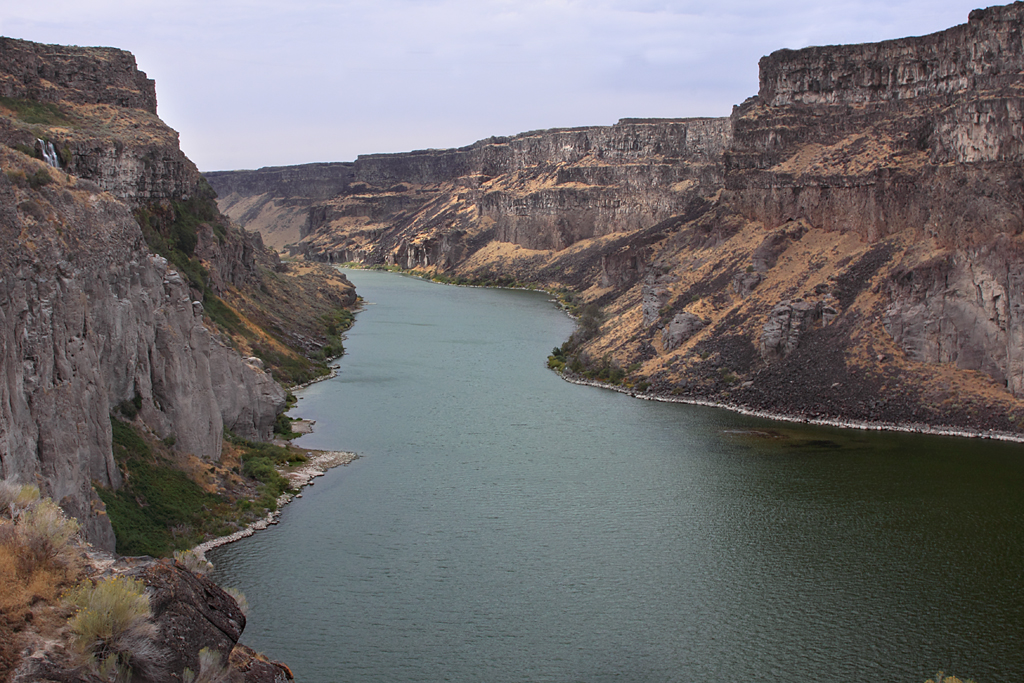
\includegraphics[width=.3\textwidth]{photos/AlanVernon.jpg}\par
\textit{Picture by Alan Vernon on Flickr.com}
\end{center}
\end{minipage}
\end{activity}

      
\label{m38730*cid7}

\summary{VPdgh}
            \nopagebreak
\label{m38730*id311034}\begin{itemize}[noitemsep]
            \label{m38730*id973}\item Daar is drie fases van materie: vaste stof, vloeistof en gas.
\label{m38730*id872}\item Diffusie is die beweging van deeltjies van 'n hoë konsentrasie na 'n lae konsentrasie. Brownbeweging is die diffusie (verspreiding) van baie deeltjies.
\label{m38730*uid80}\item Die \textbf{kinetiese teorie} van materie poog om die gedrag van materie in die verskillende fases te verduidelik.
\label{m38730*uid81}\item Die kinetiese teorie van materie stel dit dat alle materie uit \textbf{deeltjies} bestaan wat 'n sekere hoeveelheid \textbf{energie} het, wat hulle toelaat om teen verskillende snelhede te \textbf{beweeg}, afhangende van die temperatuur (energie). Daar is \textbf{ruimtes} tussen die deeltjies en ook \textbf{aantrekkingskragte} tussen die deeltjies as hulle naby aan mekaar kom.
\label{m38730*uid83}\item \textbf{Smeltpunt} is die temperatuur waarby 'n vaste stof van fase verander en 'n vloeistof word.
\label{m38730*uid84}\item \textbf{Kookpunt} is die spesifieke temperatuur waarby 'n vloeistof se fase verander om 'n gas te word. Die omgekeerde proses (verandering in fase van gas na 'n vloeistof) word \textbf{kondensasie} genoom.
\end{itemize}
\label{m38730*cid9}
            \begin{eocexercises}{Fases van materie en die kinetiese molekul\^{e}re teorie}
            \nopagebreak \noindent
\label{m38730*id311490}\begin{enumerate}[noitemsep, label=\textbf{\arabic*}. ] 
            \label{m38730*uid87}\item Gee een woord of term vir elk van die volgende beskrywings:
\label{m38730*id311506}\begin{enumerate}[noitemsep, label=\textbf{\alph*}. ] 
            \label{m38730*uid88}\item Die verandering in fase van 'n vaste stof na 'n gas.
\label{m38730*uid89}\item Die verandering in fase van vloeistof na gas.
\end{enumerate}
                \label{m38730*uid103}\item Water het 'n kookpunt van $100 ^{\circ} C$
\label{m38730*id311744}\begin{enumerate}[noitemsep, label=\textbf{\alph*}. ] 
            \label{m38730*uid104}\item Defineer 'kookpunt'.
\label{m38730*uid105}\item Watter fase verandering vind plaas wanneer 'n vloeistof kookpunt bereik?
\label{m38730*uid107}\item Gebruik die kinetiese teorie van materie en jou kennis van intermolekul\^{e}re kragte om te verduidelik waarom water van fase verander by hierdie temperatuur.
\end{enumerate}
\label{m38730*id762}\item Beskryf 'n vaste stof in terme van die kinetiese molekul\^{e}re teorie. \newline
            \label{m38730*uid108}\item Verwys na die tabel hieronder wat die smelt-en kookpunte van 'n aantal elemente aandui en beantwoord dan die vrae wat volg. (Data uit \textsl{http://www.chemicalelements.com})
    % \textbf{m38730*id311817}\par
          \begin{table}[H]
    % \begin{table}[H]
    % \\ 'id2883166' '1'
        \begin{center}
      \label{m38730*id311817}
      \begin{tabular}{|l|l|l|}\hline
\textbf{Element} & \textbf{Smeltpunt ($^{\circ} \text{C}$)} & \textbf{Kookpunt ($^{\circ} \text{C}$)} \\ \hline
        koper &
        1083 &
        2567 \\ \hline
        magnesium &
        650 &
        1107 \\ \hline
        suurstof &
        -218,4 &
        -183 \\ \hline
        koolstof &
        3500 &
        4827 \\ \hline
        helium &
        -272 &
        -268,6 \\ \hline
        swawel &
        112,8 &
        444,6 \\ \hline
    \end{tabular}
      \end{center}
\end{table}
  \label{m38730*id312057}\begin{enumerate}[noitemsep, label=\textbf{\alph*}. ] 
            \label{m38730*uid109}\item In watter fase van materie (d.w.s. vaste stof, vloeistof of gas) sal elkeen van hierdie elemente by kamertemperatuur ($25^{\circ} \text{C}$) wees?
\label{m38730*uid110}\item Watter een van hierdie elemente het die stekste kragte tussen die atome? Gee 'n rede vir jou antwoord.
\label{m38730*uid111}\item Watter een van hierdie elemente het die swakste kragte tussen die atome? Gee 'n rede vir jou antword.
\end{enumerate}
\item Voltooi die volgende submikroskopiese diagramme om te wys hoe magnesium sal lyk in die vaste stof, vloeistof en gas fase.
\begin{figure}[H]
\begin{center}
\scalebox{.8}{
\begin{pspicture}(0,0)(10,2.6)
\SpecialCoor
%\psgrid[gridcolor=lightgray]

\rput(0,0.5){\psframe(0,0)(3,2)}

\rput(3.5,0.5){\psframe(0,0)(3,2)}

\rput(7,0.5){\psframe(0,0)(3,2)}

\uput[d](1.5,0.5){solid}
\uput[d](5,0.5){liquid}
\uput[d](8.5,0.5){gas}

\end{pspicture}
}
\end{center}
\end{figure}
                \end{enumerate}

\practiceinfo
\begin{tabular}[h]{cccccc}
 (1.) l2t  &  (2.) lip  &  (3.) lim  &  (4.) lgf  &  (5.) liy  & 
\end{tabular}
\end{eocexercises}